\documentclass[10pt]{beamer}

\usetheme{default}

\usepackage[utf8]{inputenc}
\usepackage[russian]{babel}
\usepackage[OT1]{fontenc}
\usepackage{amsmath}
\usepackage{amsfonts}
\usepackage{amssymb}
\usepackage{graphicx}
\usepackage{etoolbox}
\usepackage{caption}
\usepackage{subcaption}
\captionsetup{compatibility=false}
\usepackage{booktabs}
\usepackage{array}
\usepackage{hyperref}



\makeatletter



\setbeamercolor{title}{fg=white}
\setbeamercolor{frametitle}{fg=black}
\setbeamerfont*{title}{family=\sffamily,size=\LARGE}

\setbeamerfont{page number in head/foot}{size=\scriptsize}
\setbeamertemplate{footline}[frame number]
\let\otp\titlepage
\renewcommand{\titlepage}{\otp\addtocounter{framenumber}{-1}}

\setbeamertemplate{background canvas}{%
	\ifnumequal{\c@framenumber}{0}{%
      
\includegraphics[width=\paperwidth,height=\paperheight]{images/cover.png}
   }{%
      \ifnumequal{\c@framenumber}{\inserttotalframenumber}{
         
\includegraphics[width=\paperwidth,height=\paperheight]{images/back.png}
      }{%
         % Other frames
      }%
   }%
}

\makeatother

\beamertemplatenavigationsymbolsempty

\author{Нестеров Павел}
\title{\newline \newline \newline Лекция n3 \\ Глубокие нейронные сети}

\begin{document}

\begin{frame}[plain]
\titlepage
\end{frame}

\begin{frame}{План лекции}
\tableofcontents
\end{frame}


\section{Вспоминаем пройденное}


\begin{frame}{Многоснойная нейронная сеть прямого распространения}

\begin{figure}[h!]
  \centering
  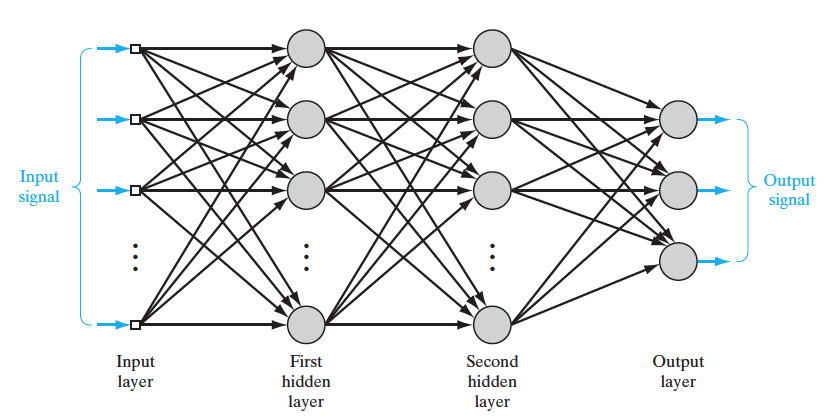
\includegraphics[width=1\textwidth]{images/mlp.png}
  \caption{Архитектура сети с двумя скрытыми слоями\footnote{Neural Networks and Learning Machines (3rd Edition), Simon O. Haykin}}
\end{figure}

\end{frame}


\begin{frame}{Ограниченная машина Больцмана}

\begin{columns}
    \column{0.4\textwidth}
	
	\begin{figure}[h!]
		\centering
  		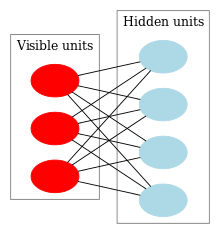
\includegraphics[width=1\textwidth]{images/rbm_graph.png}
	\end{figure} 
    
    \column{0.6\textwidth}
	
	\begin{eqnarray*}
		\Delta w_{ij} &=& \eta\left( M\left[v_i^{(k)} h_j \right]_{\textsc{data}} - M\left[v_i h_j\right]_{\textsc{model}} \right) \\
		\Delta a_i &=& \eta\left( v_i^{(k)} - M\left[v_i\right]_{\textsc{model}} \right) \\
		\Delta b_j &=& \eta\left( M\left[h_j \right]_{\textsc{data}} - M\left[h_j\right]_{\textsc{model}} \right)
	\end{eqnarray*}
\end{columns}

\end{frame}


\begin{frame}{Contrastive-divergence}

\begin{figure}[h!]
  \centering
  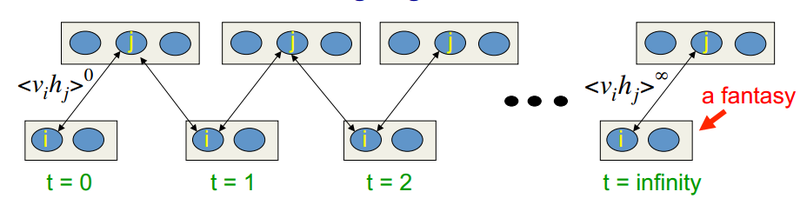
\includegraphics[width=1\textwidth]{images/cd.png}
  \caption{Процесс сбора достаточной статистики\footnote{https://class.coursera.org/neuralnets-2012-001/lecture}}
\end{figure}

\begin{eqnarray*}
\frac{\partial \ln P\left(v^{(k)}\right)}{\partial w_{ij}} &=& \sum_t^M v_i^{(k)} h_j^{(t)} P\left( h^{(t)} | v^{(k)} \right) - \sum_r^N \sum_t^M v_i^{(r)} h_j^{(t)} P\left( h^{(t)}, v^{(k)} \right) \\
&=& M\left[v_i^{(k)} h_j \right]_{\textsc{data}} - M\left[v_i h_j\right]_{\textsc{model}}
\end{eqnarray*}

\end{frame}


\begin{frame}{Семплирование по Гиббсу}

Семплирование по Гиббсу не требуется явно выраженное совместное распределение, а нужны лишь условные вероятности для каждой переменной, входящей в распределение. Алгоритм на каждом шаге берет одну случайную величину и выбирает ее значение при условии фиксированных остальных. Можно показать, что последовательность получаемых значений образуют возвратную цепь Маркова, устойчивое распределение которой является как раз искомым совместным распределением.

\begin{itemize}
	\item $p_{0} = \sum_t^M v_i^{(k)} h_j^{(t)} P\left( h^{(t)} | v^{(k)} \right)$ - это оценка реального распределения основываясь на данных
	\item $p_{k \rightarrow \infty} = \sum_r^N \sum_t^M v_i^{(r)} h_j^{(t)} P\left( h^{(t)}, v^{(r)}\right)$ - оценка реального распределения с помощью семплирования по Гиббсу, которое несомненно когда то сойдется в реальному\footnote{http://www.ini.rub.de/data/documents/tns/masterthesis\underline{ }janmelchior.pdf}
	\item $\frac{\partial \ln P\left(v^{(k)}\right)}{\partial w_{ij}} = p_0 - p_{k \rightarrow \infty} = 0$
\end{itemize}

\end{frame}


\begin{frame}{Зачем нам глубокие сети?}

\begin{figure}[h!]
  \centering
  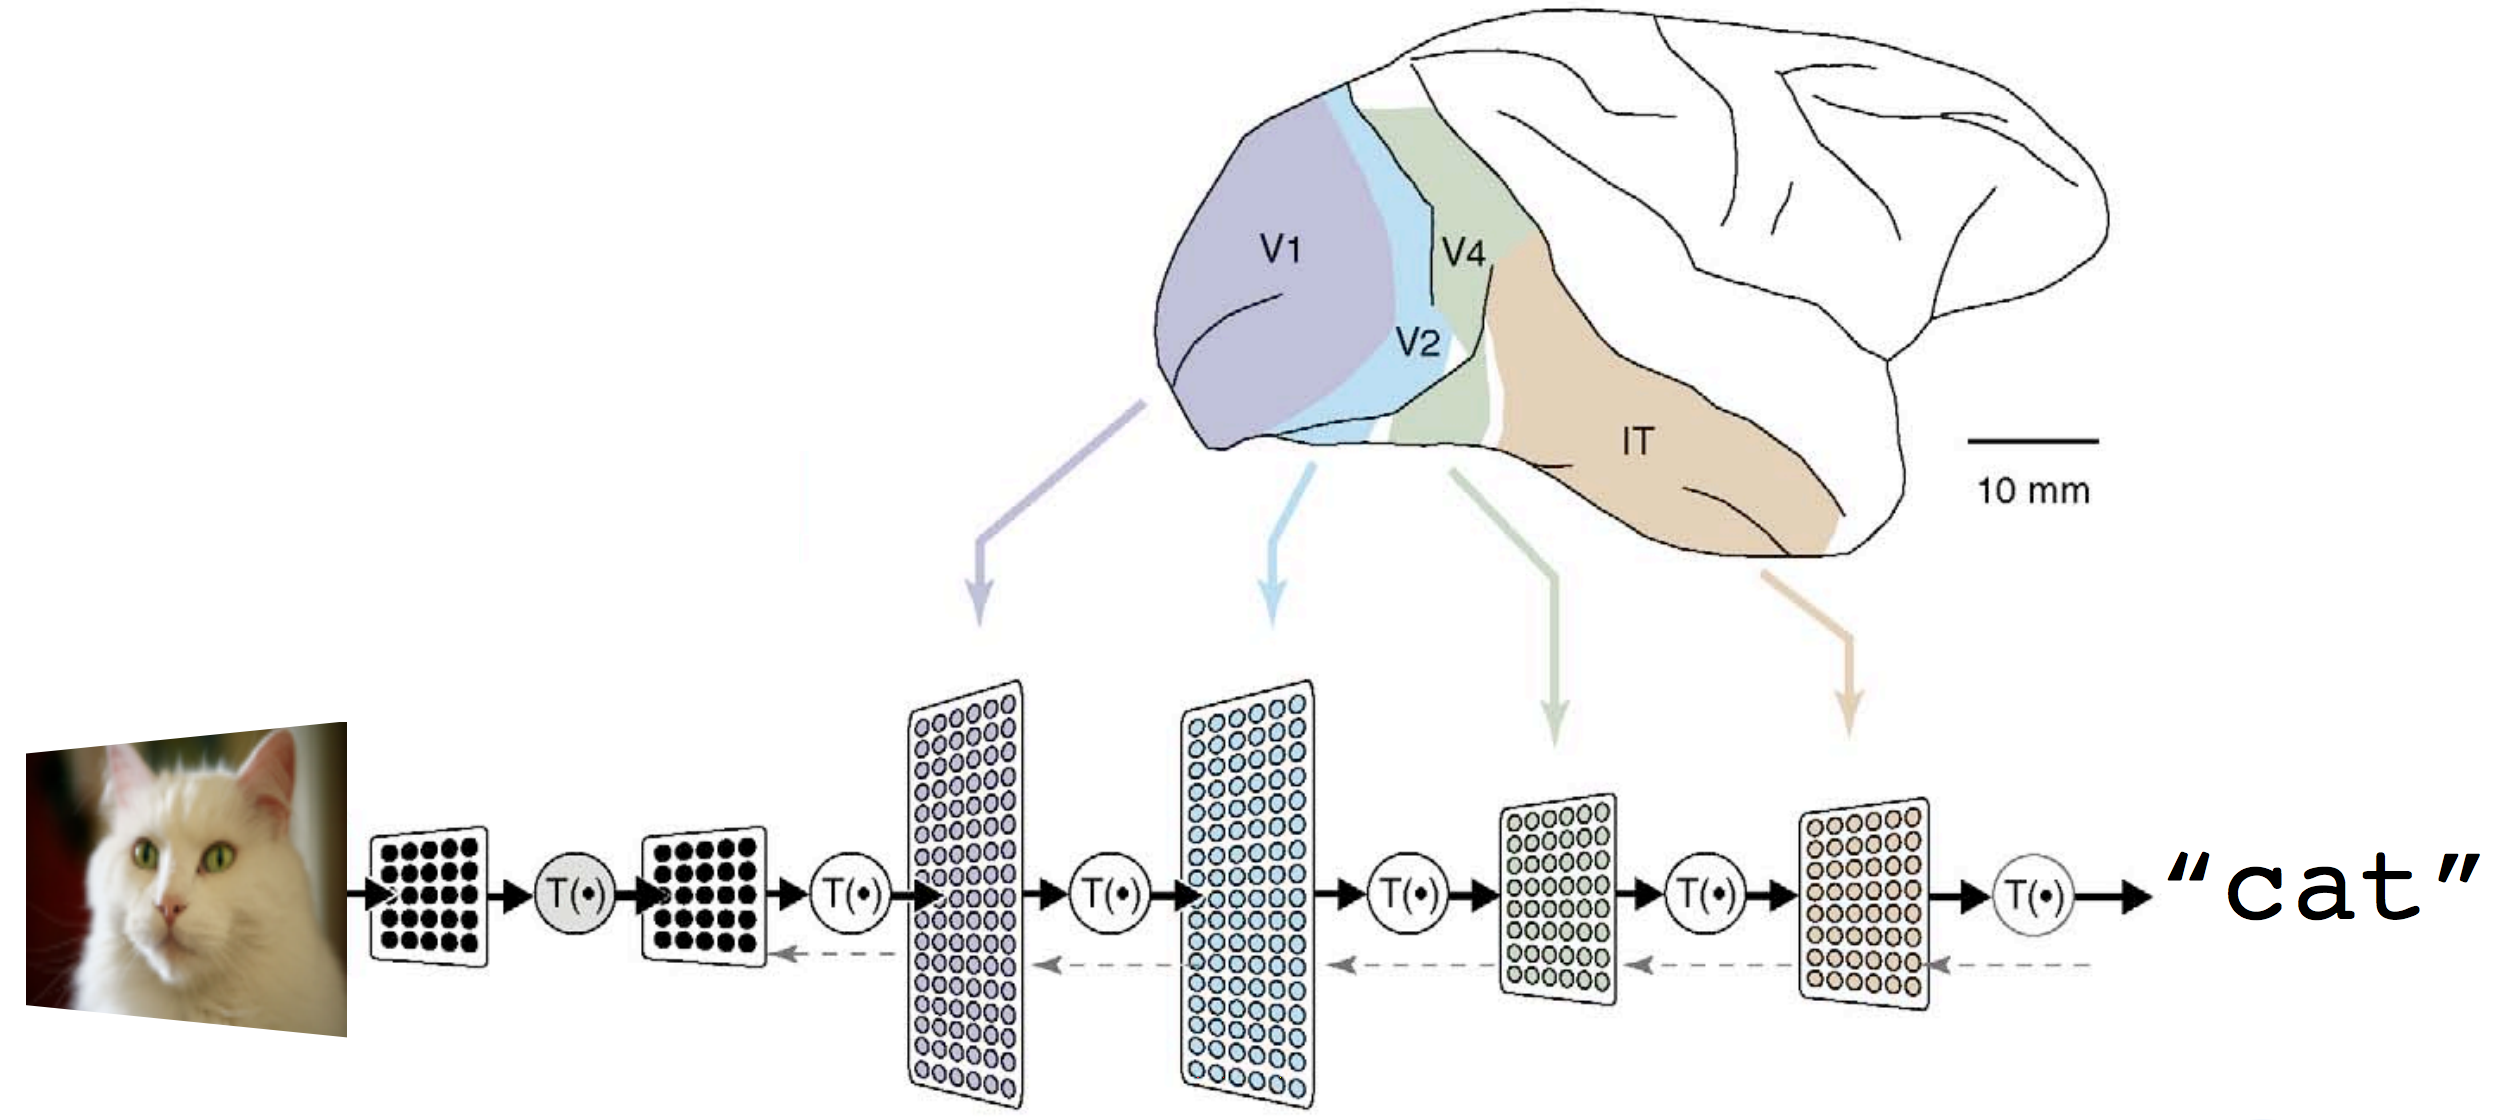
\includegraphics[width=0.6\textwidth]{images/deepnet1.png}
  \caption{Глубокая нейронная сеть\footnote{Из предентации Scale Deep Learning, Jeff Dean}}
\end{figure}

\begin{itemize}
	\item Согласно стандартной модели зрительной коры головного мозга\footnote{Hubel and Wiesel 1962; Serre et al. 2005; Ranzato et al.
2007} считается, что каждый следующий нейронный слой выучивает новый уровень абстракции данных \footnote{Palmer 1999; Kandel et al. 2000} (например штрихи, пятна, поверхности, объекты);
	\item мало того, было показано, что добавление нового слоя в модель улучшает нижнюю вариационную границу логарифма правдоподобия генеративной модели\footnote{Learning multiple layers of representation (G. Hinton, 2007)}.
\end{itemize}

\end{frame}


\section{Проблемы алгоритма обратного распространения ошибки}

\begin{frame}{Паралич сети, эксперимент}

\begin{table}[h]
\begin{tabular}{|l|l|l|l|l|l|l|}
\hline
input = 841 & layer -5 & layer -4 & layer -3 & layer -2 & layer -1 & output \\ \hline
neurons     & 100      & 100      & 100      & 100      & 100      & 26     \\ \hline
\end{tabular}
\end{table}

\begin{figure}[h!]
  \centering
  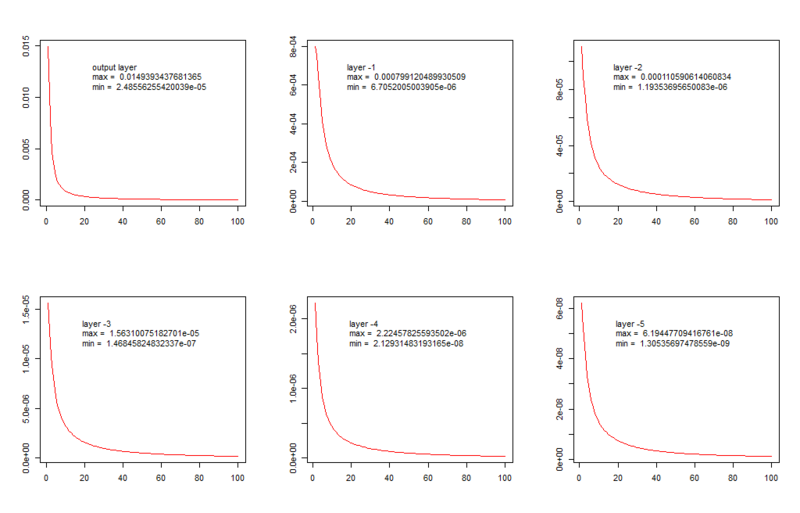
\includegraphics[width=1\textwidth]{images/bp_hist.png}
\end{figure}


\end{frame}


\begin{frame}{Backprop, прямой проход}

\begin{columns}
    \column{0.4\textwidth}	
	\begin{figure}[h!]
		\centering
		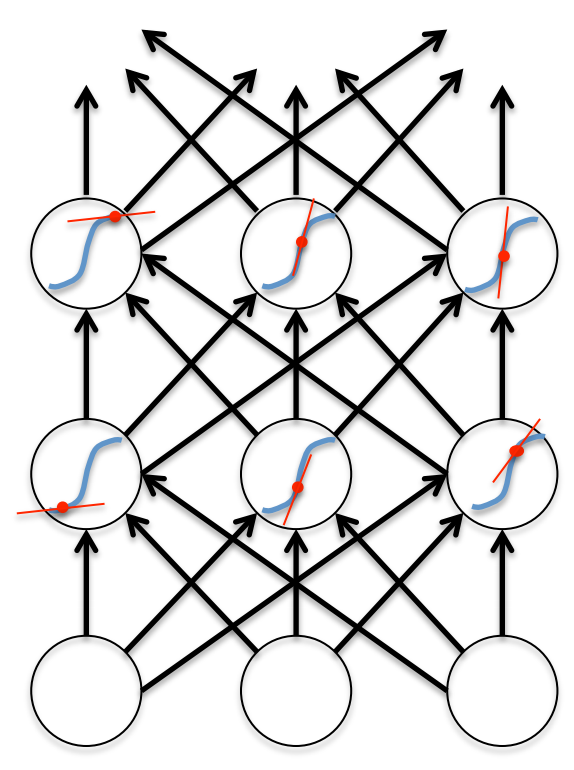
\includegraphics[width=1\textwidth]{images/bp_f.png}
	\end{figure}
    
    \column{0.6\textwidth}
	\begin{itemize}
		\item $y^{(n)}_k = \sigma^{(n)}_k\left(\sum^{N_{n-1}}_{i=0} w^{(n)}_{ij}x^{(n)}_i\right)$
		\item выходные значения каждого нейрона лежат в строго заданных пределах
	\end{itemize}	
\end{columns}
\textit{Прямой проход в нейросети\footnote{https://class.coursera.org/neuralnets-2012-001/lecture}}

\end{frame}


\begin{frame}{Backprop, обратный проход, \#1}

\begin{figure}[h!]
  \centering
  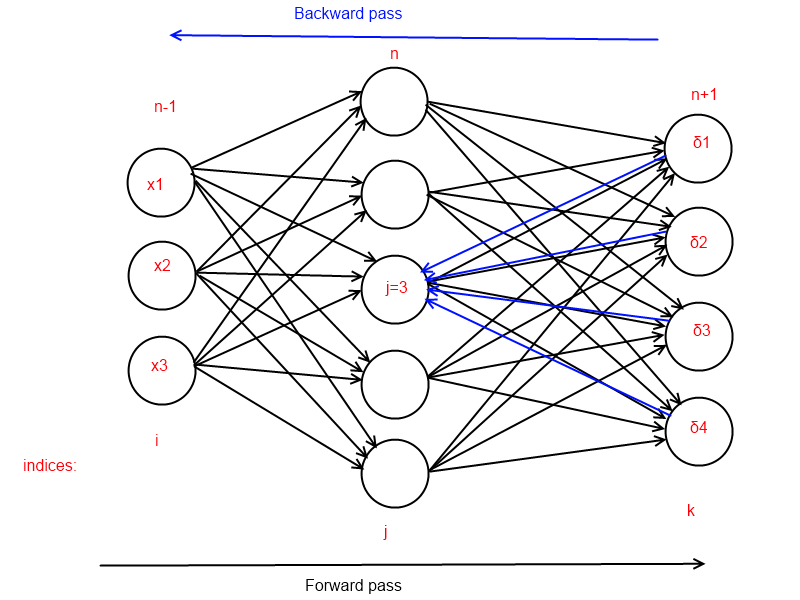
\includegraphics[width=0.9\textwidth]{images/f_b_pass.png}
  \caption{Схема прямого (нелинейного) и обратного (линейного) распространения сигнала в сети}
\end{figure}

\end{frame}


\begin{frame}{Backprop, обратный проход, \#2}

Вспомним формулу градиента для скрытых слоев:
\begin{equation*}
\dfrac{\partial E}{\partial w^{(n)}_{ij}} = x^{(n - 1)}_i \sum_k w^{(n + 1)}_{ik} \dfrac{\partial E}{\partial z^{(n + 1)}_k}  \dfrac{\partial y^{n}_{j}}{\partial z^{n}_{j}}
\end{equation*}
Выполнив замену $\delta_k^{(n)} = \frac{\partial E}{\partial w^{(n)}_{ij}}$, получим следующее:
\begin{equation*}
\dfrac{\partial E}{\partial w^{(n)}_{ij}} = x^{(n - 1)}_i \dfrac{\partial y^{n}_{j}}{\partial z^{n}_{j}} \sum_k w^{(n + 1)}_{ik} \delta_k^{(n)} = \sum_k c_k \delta_k^{(n)}
\end{equation*}
\begin{itemize}
	\item в итоге получилась линейная функция от $\delta_k^{(n)}$.
	\item $\delta_k^{(n)}$ - локальный градиент/ошибка нейрона \textit{(она как раз и распространяется обратно)}
\end{itemize}

\end{frame}


\begin{frame}{Backprop, затухание градиента, \#1}

Рассмотрим в качестве функции активации функцию логистического сигмоида:
\begin{eqnarray*}
y(z) &=& \frac{1}{1 + e^{-z}} \\
\frac{\partial y(z)}{\partial z} &=& y(z)\cdot \left( 1 - y(z) \right)
\end{eqnarray*}
Построим график значений производной:
\begin{columns}
    \column{0.5\textwidth}	
	\begin{figure}[h!]
  		\centering
  		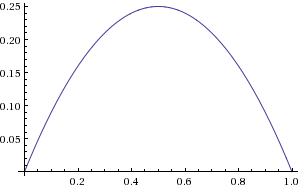
\includegraphics[width=1\textwidth]{images/logsigm_plot.png}
	\end{figure}
    
    \column{0.6\textwidth}
	\begin{itemize}
		\item максимум равен $\sigma_{\textsc{max}} = 0.25 = \frac{1}{4}$
	\end{itemize}	
\end{columns}

\end{frame}


\begin{frame}{Backprop, затухание градиента, \#2}

Рассмотрим простую сеть:
\begin{figure}[h!]
	\centering
  	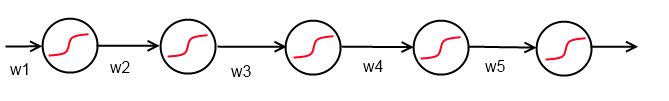
\includegraphics[width=1\textwidth]{images/simple_net.png}
\end{figure}
Вычислим градиенты весов для $E(\vec y, \vec t) = \frac{1}{2} \sum_j(y_j - t_j)^2$:
\begin{eqnarray*}
\dfrac{\partial E}{\partial w^{(n)}_{ij}} &=& x_i^{(n - 1)} \dfrac{\partial E}{\partial y^{(n)}_j} \dfrac{\partial y^{(n)}_j}{\partial z^{(n)}_j} \\
\frac{\partial E}{\partial w_5} &=& ???
\end{eqnarray*}

\end{frame}


\begin{frame}{Backprop, затухание градиента, \#3}

Рассмотрим простую сеть:
\begin{figure}[h!]
	\centering
  	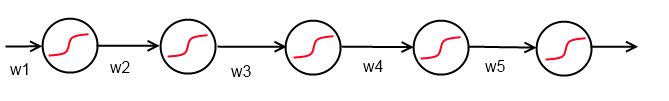
\includegraphics[width=1\textwidth]{images/simple_net.png}
\end{figure}
Вычислим градиенты весов для $E(\vec y, \vec t) = \frac{1}{2} \sum_j(y_j - t_j)^2$:
\begin{eqnarray*}
	\dfrac{\partial E}{\partial w^{(n)}_{ij}} &=& x^{(n - 1)}_i \sum_k w^{(n + 1)}_{ik} \dfrac{\partial E}{\partial z^{(n + 1)}_k}  \dfrac{\partial y^{n}_{j}}{\partial z^{n}_{j}} \\
\frac{\partial E}{\partial w_5} &=& y_4 (y_5 - t) y_5 (1 - y_5) \leq y_4 (y_5 - t) \frac{1}{4} \\
\frac{\partial E}{\partial w_4} &=& ???
\end{eqnarray*}
	
\end{frame}


\begin{frame}{Backprop, затухание градиента, \#4}

Рассмотрим простую сеть:
\begin{figure}[h!]
	\centering
  	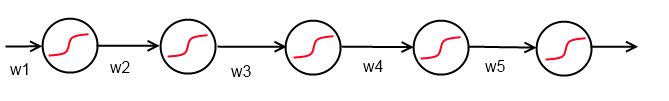
\includegraphics[width=1\textwidth]{images/simple_net.png}
\end{figure}
Вычислим градиенты весов для $E(\vec y, \vec t) = \frac{1}{2} \sum_j(y_j - t_j)^2$:
\begin{eqnarray*}
\frac{\partial E}{\partial w_5} &=& y_4 (y_5 - t) y_5 (1 - y_5) \leq y_4 (y_5 - t) \frac{1}{4} \\
\frac{\partial E}{\partial w_4} &=& y_3 w_5 (y_5 - t) y_4 (1 - y_4) y_5 (1 - y_5) \leq y_3 w_5 (y_5 - t) \frac{1}{4^2} \\
\frac{\partial E}{\partial w_3} &\leq& y_2 w_4 w_5 (y_5 - t) \frac{1}{4^3} \\
\frac{\partial E}{\partial w_2} &\leq& y_1 w_3 w_4 w_5 (y_5 - t) \frac{1}{4^4} \\
\frac{\partial E}{\partial w_1} &\leq& x w_2 w_3 w_4 w_5 (y_5 - t) \frac{1}{4^5}
\end{eqnarray*}
	
\end{frame}


\begin{frame}{Backprop, паралич сети, выводы}

\begin{itemize}
	\item значение градиента затухает экспоненциально в принципе $\Rightarrow$ сходимость замедляется
	\item при малых значениях весов этот эффект усиливается
	\item при больших значения весов значение градиента может экспоненциально возрастать $\Rightarrow$ алгоритм расходится
	\item не глубокие сети не сильно страдают от этого
\end{itemize}

\end{frame}

\section{Предобучение глубокой нейронной сети}

\begin{frame}{Проблема паралича сети, визуализация}

\begin{figure}
        \centering
        \begin{subfigure}[b]{0.5\textwidth}
                
\includegraphics[width=0.9\textwidth]{images/cat.png}
                \caption{Исходное изображение}                
        \end{subfigure}%  
        \begin{subfigure}[b]{0.5\textwidth}
                
\includegraphics[width=0.9\textwidth]{images/cat_noised.png}
                \caption{Образ в первом скрытом слое}                
        \end{subfigure}       
        \caption{Оригинал и его образ в первом скрытом слое нейронной сети при количестве нейронов нем равном размерности входного образа при инициализации весов $w_{ij} \sim \mathcal{N}\left(0, 0.01\right)$}
\end{figure}

\end{frame}


\begin{frame}{Решение проблемы паралича сети, идея, \#1}

\begin{itemize}
	\item А что если инициализировать веса таким образом, что бы образ оригинального изображения в скрытом пространстве описывал бы прообраз максимально точно?
	\item \textit{Есть идеи?}
\end{itemize}

\end{frame}


\begin{frame}{Решение проблемы паралича сети, идея, \#2}

\begin{itemize}
	\item А что если инициализировать веса таким образом, что бы образ оригинального изображения в скрытом пространстве описывал бы прообраз максимально точно?
	\item Именно это и делает ограниченная машина Больцмана
\end{itemize}

\begin{figure}[h!]
  \centering
  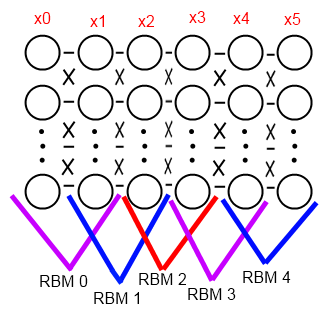
\includegraphics[width=0.6\textwidth]{images/rbm_pretrain.png}
\end{figure}

\end{frame}


\begin{frame}{Жадный алгоритм предобучения}
Собственно алгоритм
\begin{enumerate}
	\item последовательно натренировать каждую пару слоев в глубокой сети (возможно кроме первого и второго скрытого слоя от выходного слоя);
	\item осуществить тонкую настройку весов, используя алгоритм обратного распространения ошибки (fine turning).
\end{enumerate}

Некоторые важные преимущества:
\begin{itemize}
	\item скорость сходимости;
	\item качество (в смысле выбранной меры);
	\item возможно использовать не только размеченные образы для обучения с учителем (\textit{как? примеры?})
\end{itemize}

\end{frame}


\section{Другие виды глубоких сетей}

\begin{frame}{Deep directed network}

\begin{figure}[h!]
  \centering
  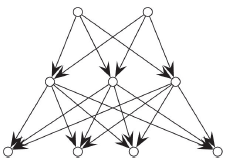
\includegraphics[width=0.4\textwidth]{images/ddn.png}
\end{figure}
Для сети с одним видимым слоем и тремя скрытыми функция правдоподобия выглядит следующим образом:
\begin{eqnarray*}
p(h_1, h_2, h_3, v | W) &=& \prod_i \text{Ber}\left(v_i | \sigma\left(h_1^T w_{0i}\right)\right) \cdot \prod_j \text{Ber}\left(h_{1j} | \sigma\left(h_2^T w_{1i}\right)\right) \cdot \\
& & \cdot \prod_k \text{Ber}\left(h_{2k} | \sigma\left(h_3^T w_{2i}\right)\right) \cdot \prod_l \text{Ber}\left(h_{3l} | w_{3l}\right)
\end{eqnarray*}

\end{frame}


\begin{frame}{Deep Boltzmann machine}

\begin{figure}[h!]
  \centering
  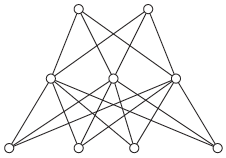
\includegraphics[width=0.4\textwidth]{images/dbm.png}
\end{figure}
Для сети с одним видимым слоем и тремя скрытыми функция правдоподобия выглядит следующим образом:
\begin{eqnarray*}
p(h_1, h_2, h_3, v | W) &=& \frac{1}{Z} \cdot \exp\left( \sum_{ij} v_i h_{ij} w_{1ij} + \right. \\
& &\left. + \sum_{jk} h_{1j} h_{2k} w_{2jk} + \sum_{kl} h_{2k} h_{3l} w_{3kl} \right)
\end{eqnarray*}

\end{frame}


\begin{frame}{Deep belief network}

\begin{figure}[h!]
  \centering
  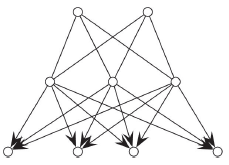
\includegraphics[width=0.4\textwidth]{images/dbn.png}
\end{figure}
Для сети с одним видимым слоем и тремя скрытыми функция правдоподобия выглядит следующим образом:
\begin{eqnarray*}
p(h_1, h_2, h_3, v | W) &=& \prod_i \text{Ber}\left(v_i | \sigma\left(h_1^T w_{0i}\right)\right) \cdot \prod_j \text{Ber}\left(h_{1j} | \sigma\left(h_2^T w_{1i}\right)\right) \cdot \\
& & \cdot \frac{1}{Z} \exp\left( \sum_{kl} h_{2k} h_{3l} w_{3kl} \right)
\end{eqnarray*}

\end{frame}


\begin{frame}{Autoencoder}

\begin{figure}[h!]
  \centering
  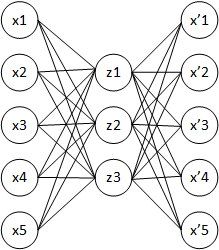
\includegraphics[width=0.4\textwidth]{images/ae.png}
  \caption{Архитектура автоассоциатора: при обучении стремятся получить выходной вектор x' наиболее близким к входному вектору x}
\end{figure}

\end{frame}


\begin{frame}{Deep autoencoder}

\begin{figure}[h!]
  \centering
  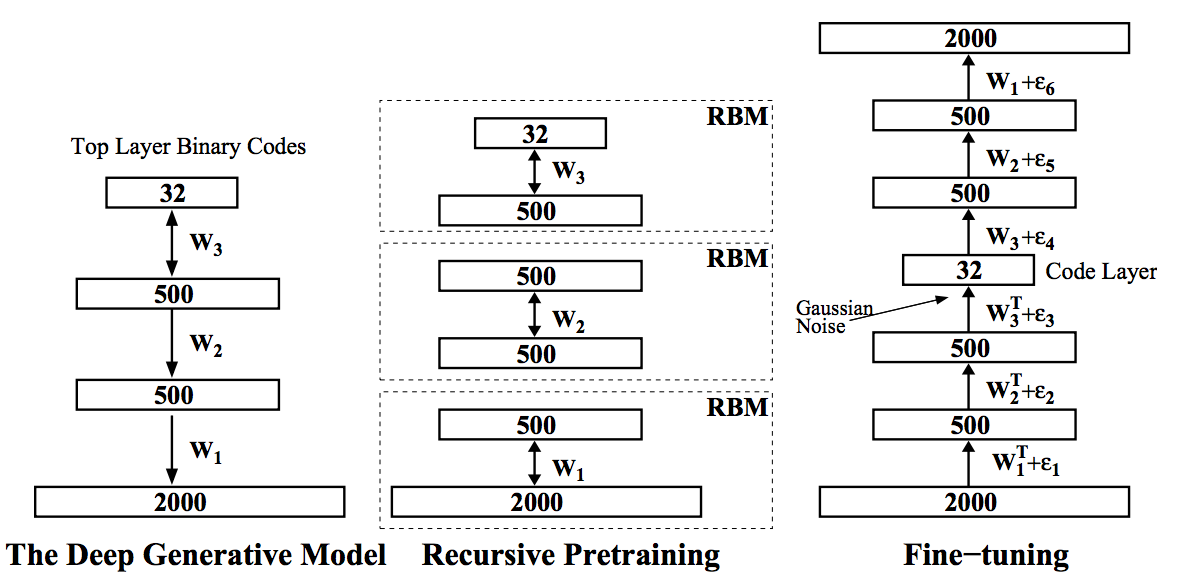
\includegraphics[width=1\textwidth]{images/dae.png}
  \caption{Semantic hashing\footnote{R. Salakhutdinov, G. Hinton}}
\end{figure}

\end{frame}


\begin{frame}{Discriminative Restricted Boltzmann Machines}

\begin{figure}[h!]
  \centering
  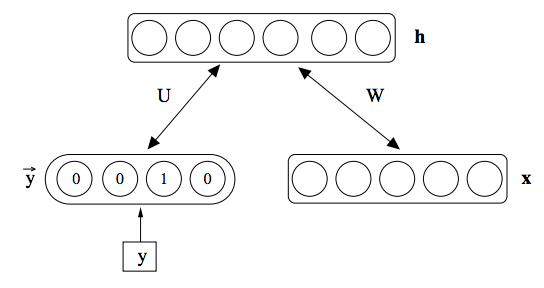
\includegraphics[width=1\textwidth]{images/drbm.png}
  \caption{Classification using Discriminative Restricted Boltzmann Machines\footnote{H. Larochelle, Y. Bengio}}
\end{figure}

\end{frame}


\begin{frame}{Deep Discriminative Restricted Boltzmann Machines}

\begin{figure}[h!]
  \centering
  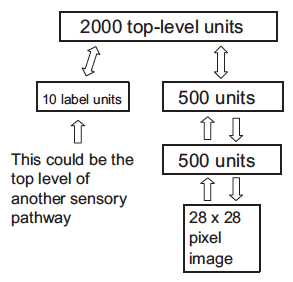
\includegraphics[width=0.6\textwidth]{images/ddrbm.png}
  \caption{RBM for MNIST\footnote{G. Hinton}}
\end{figure}

\end{frame}


\begin{frame}{Multimodal Deep Boltzmann Machine}

\begin{figure}[h!]
  \centering
  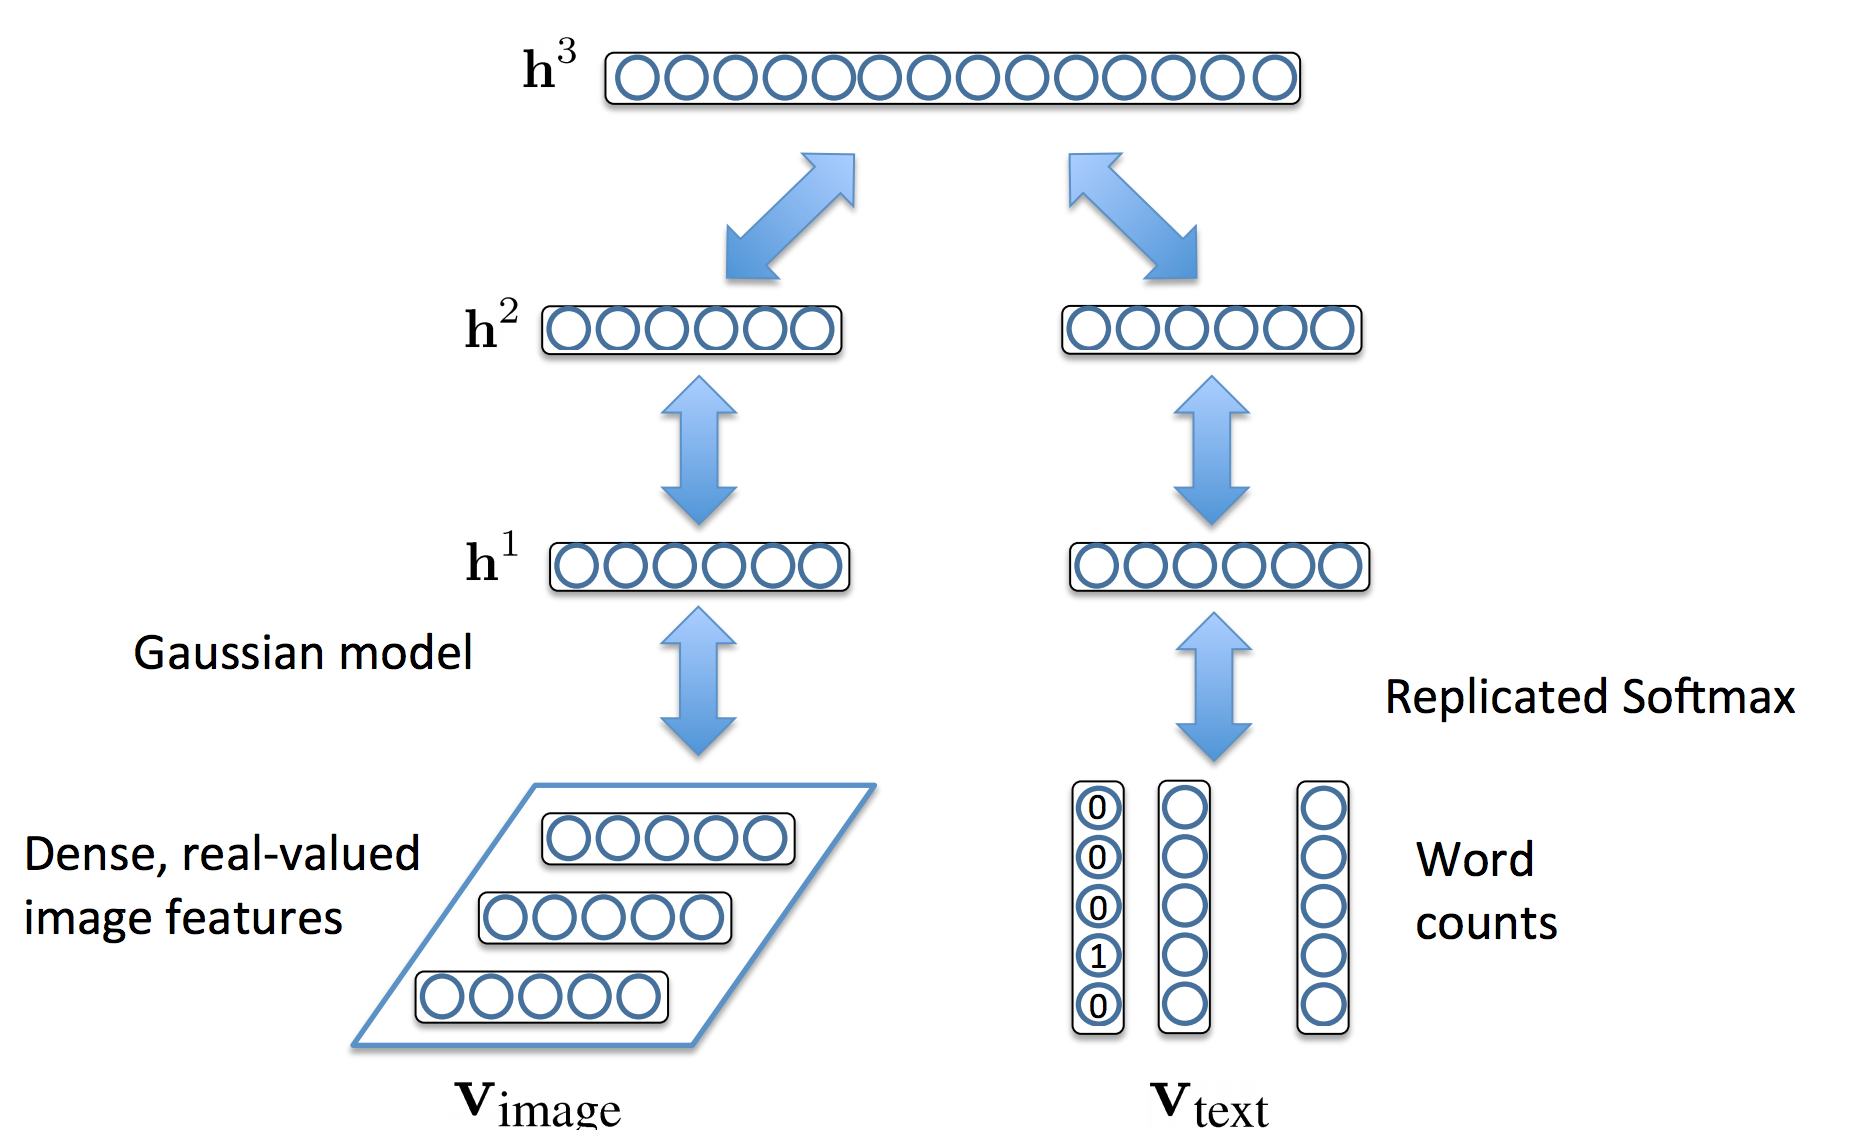
\includegraphics[width=1\textwidth]{images/mmdbm.png}
  \caption{Image + Text \footnote{Srivastava, Salakhutdinov, NIPS 2012},\\ \url{http://videolectures.net/kdd2014_salakhutdinov_deep_learning/}}
\end{figure}

\end{frame}


\begin{frame}{Recurrent Neural Network}

\begin{figure}[h!]
  \centering
  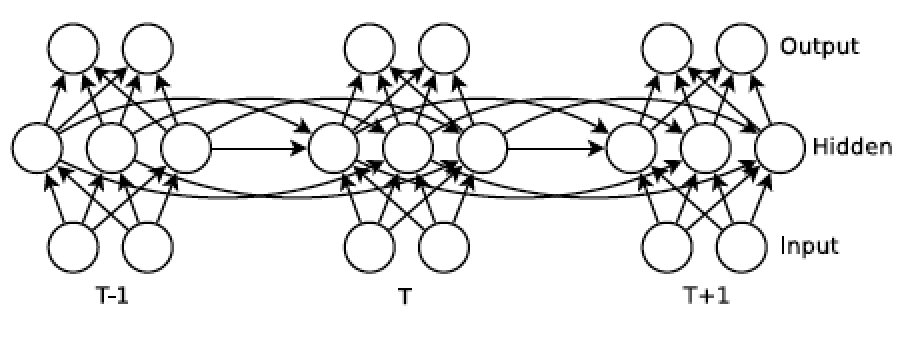
\includegraphics[width=1\textwidth]{images/rnn.png}
  \caption{RNN - это глубокая нейросеть с общими весами во времени \footnote{Generating Text with Recurrent Neural Networks, Sutskever, Martens, Hinton}}
\end{figure}

\end{frame}


\begin{frame}{Convolutional neural network}

\begin{figure}[h!]
  \centering
  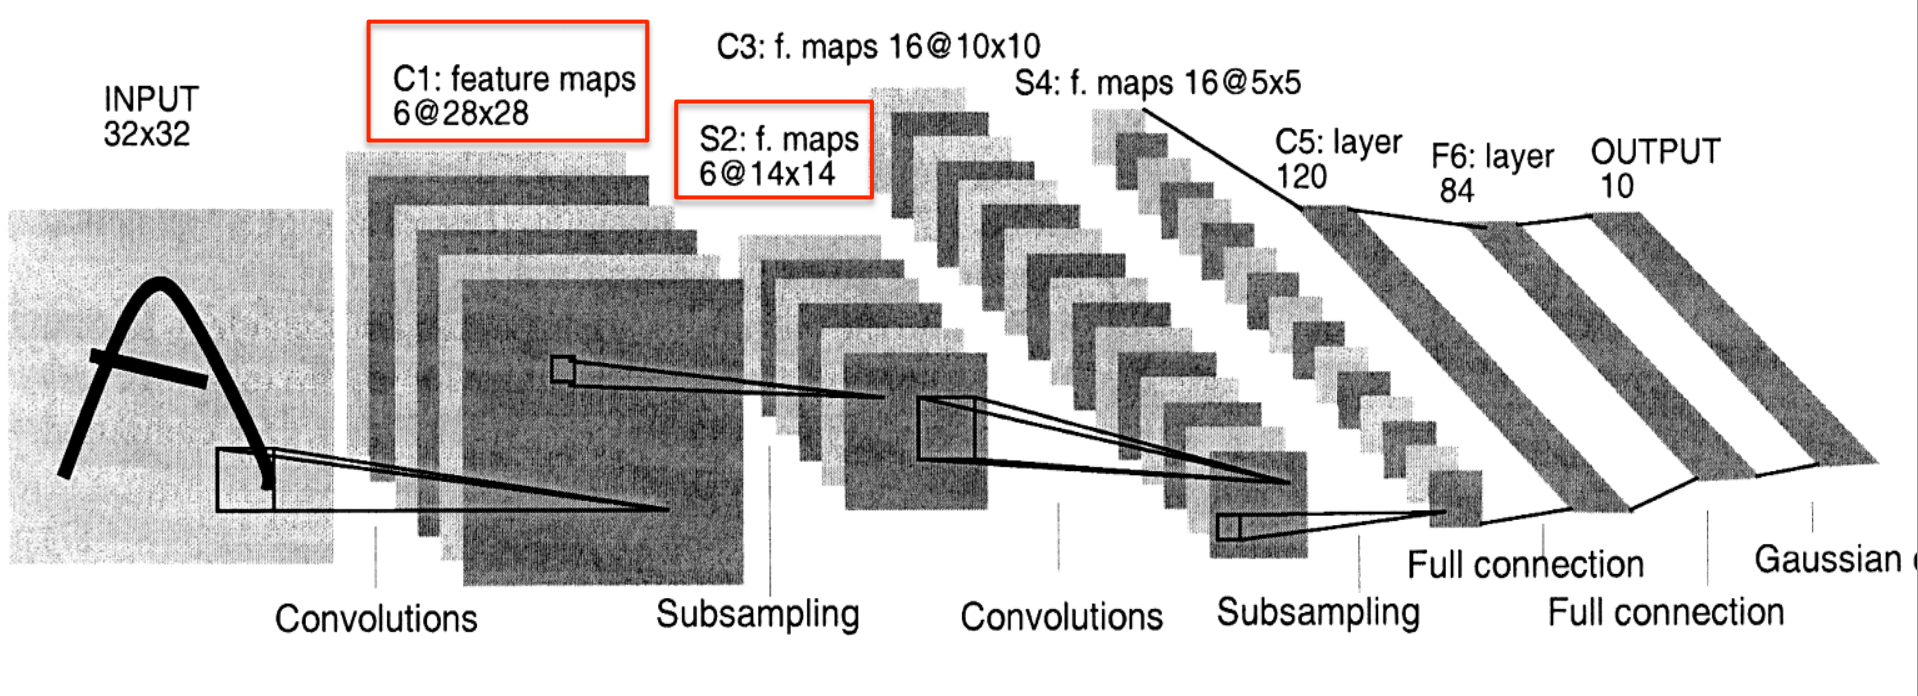
\includegraphics[width=1\textwidth]{images/cnn.png}
  \caption{LeNet for MNIST\footnote{Y. LeCunn}}
\end{figure}

\begin{itemize}
	\item lenet.gif
\end{itemize}

\end{frame}

\section{Некоторые практические применения глубоких сетей}

\begin{frame}{Сжатие размерности пространства, PCA}

\begin{columns}
    \column{0.45\textwidth}
	
	\begin{figure}[h!]
		\centering
  		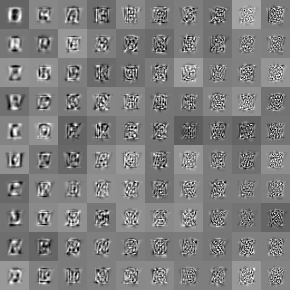
\includegraphics[width=1\textwidth]{images/pca1.png}
	\end{figure} 
    
    \column{0.45\textwidth}
	
	\begin{figure}[h!]
		\centering
  		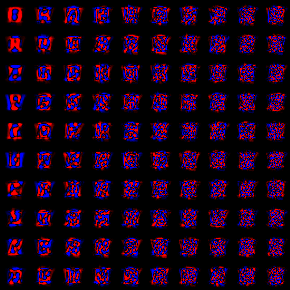
\includegraphics[width=1\textwidth]{images/pca2.png}
	\end{figure} 
	
\end{columns}

\end{frame}

\begin{frame}{Сжатие размерности пространства, RBM}

\begin{columns}
    \column{0.45\textwidth}
	
	\begin{figure}[h!]
		\centering
  		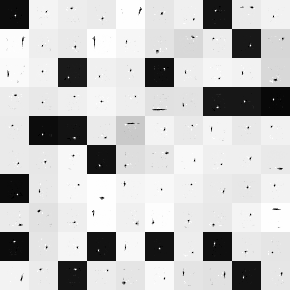
\includegraphics[width=1\textwidth]{images/rbm1.png}
	\end{figure} 
    
    \column{0.45\textwidth}
	
	\begin{figure}[h!]
		\centering
  		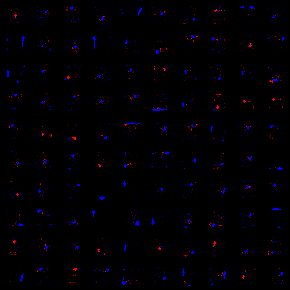
\includegraphics[width=1\textwidth]{images/rbm2.png}
	\end{figure} 
	
\end{columns}

\begin{itemize}
	\item rbm\underline{ }features*.png
\end{itemize}

\end{frame}


\begin{frame}{Learning	Similarity	Measures}

\begin{figure}[h!]
	\centering
	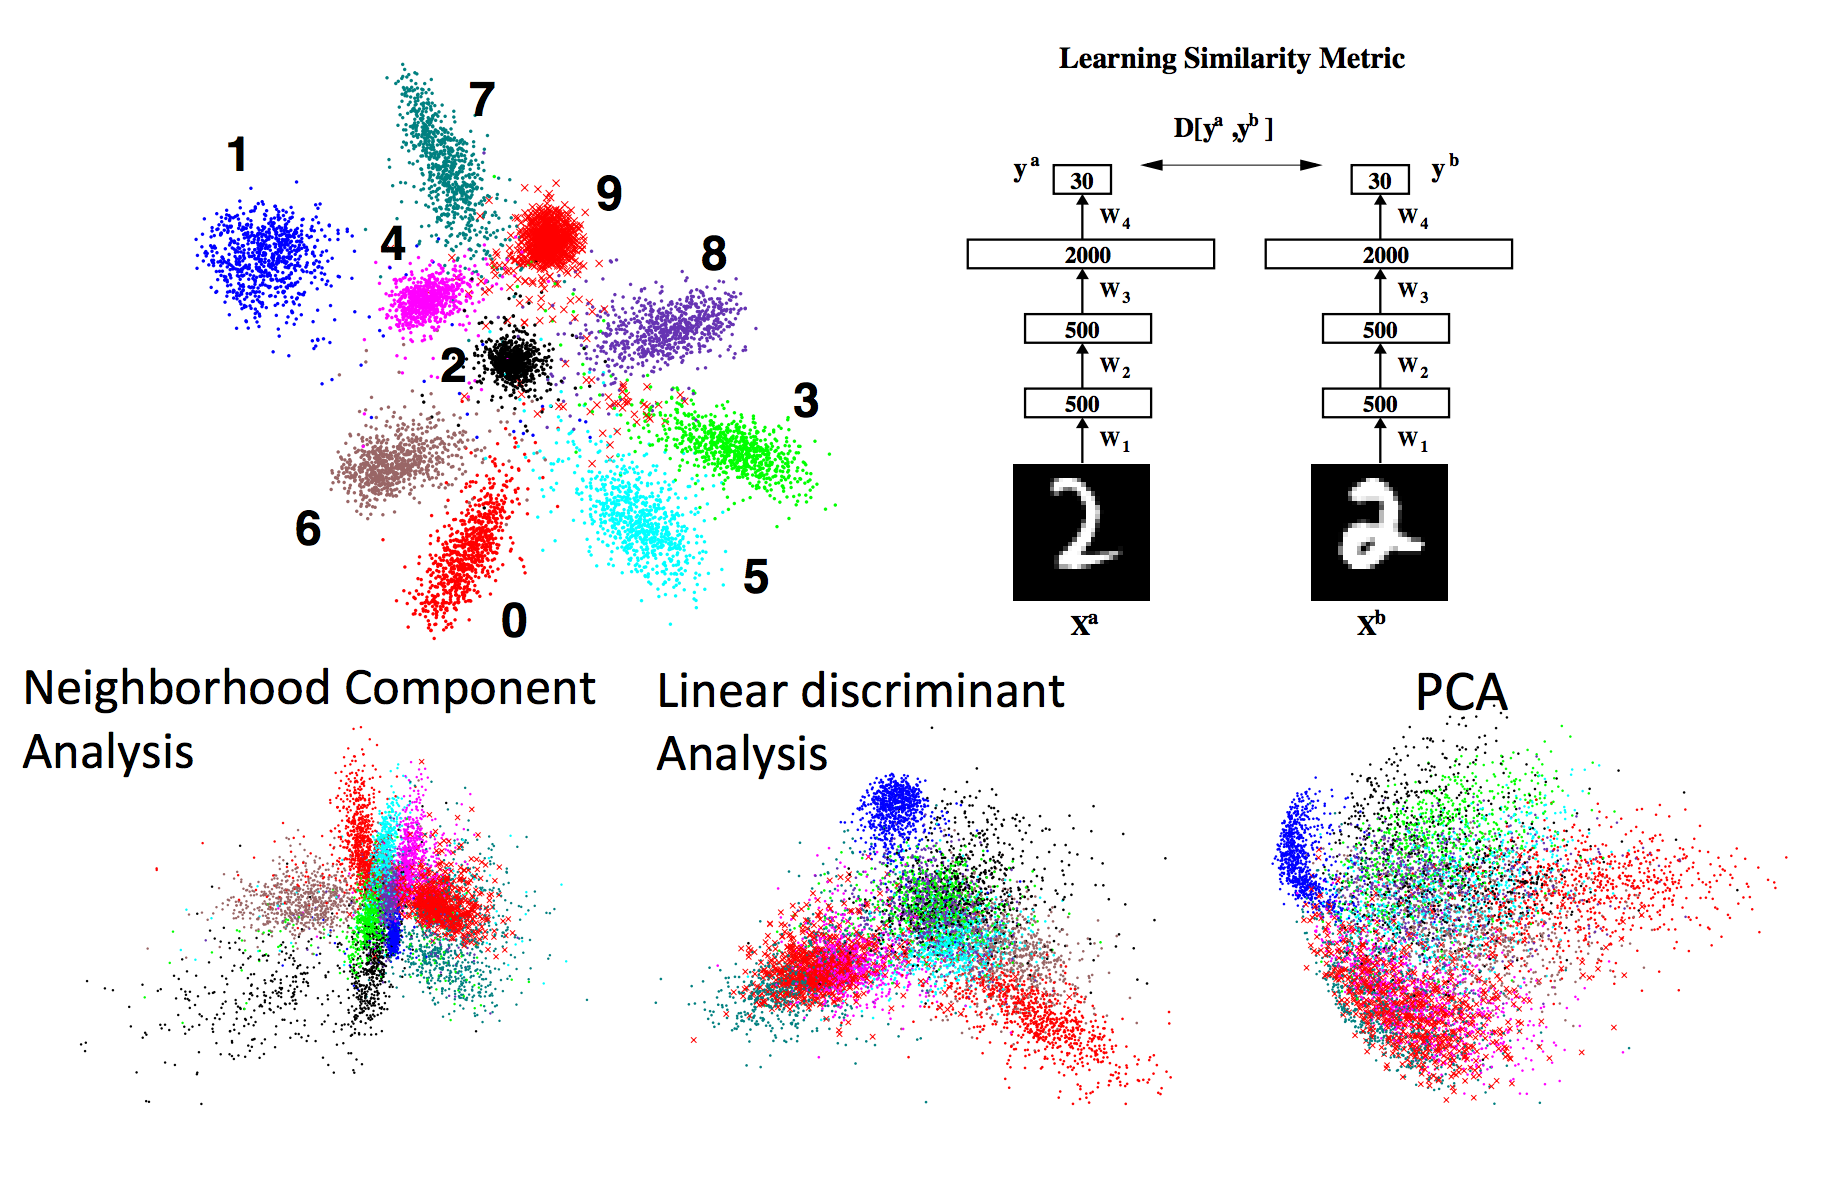
\includegraphics[width=0.9\textwidth]{images/learn_sim.png}
	\caption{New similarities in practice \footnote{Salakhutdinov and Hinton, AI and Statistics 2007},\\ \url{http://videolectures.net/kdd2014_salakhutdinov_deep_learning/}}
\end{figure} 

\end{frame}


\begin{frame}{Neurolinguistic model}


\begin{figure}[h!]
	\centering
	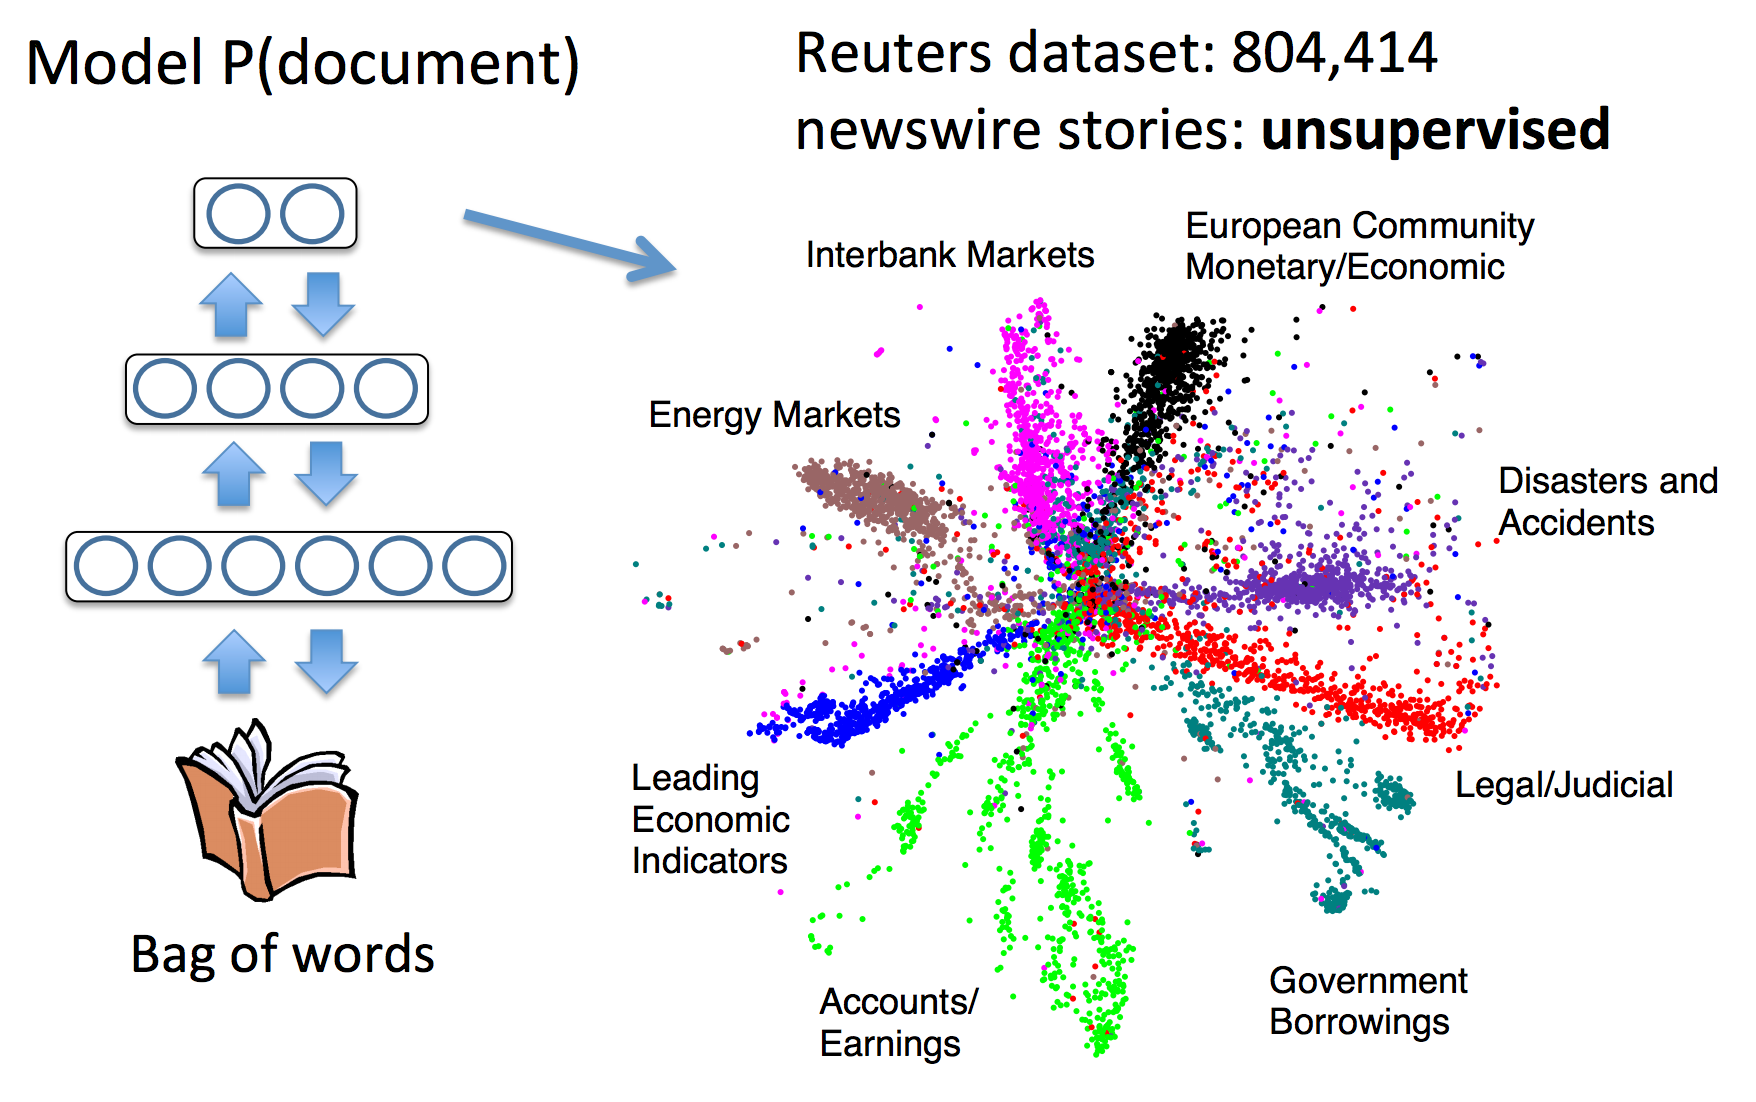
\includegraphics[width=1\textwidth]{images/neurolinguistic.png}
	\caption{Deep generative model \footnote{Hinton, Salakhutdinov, Science 2006},\\ \url{http://videolectures.net/kdd2014_salakhutdinov_deep_learning/}}
\end{figure} 

\end{frame}


\begin{frame}{Multimodal data, \#1}

\begin{figure}[h!]
	\centering
	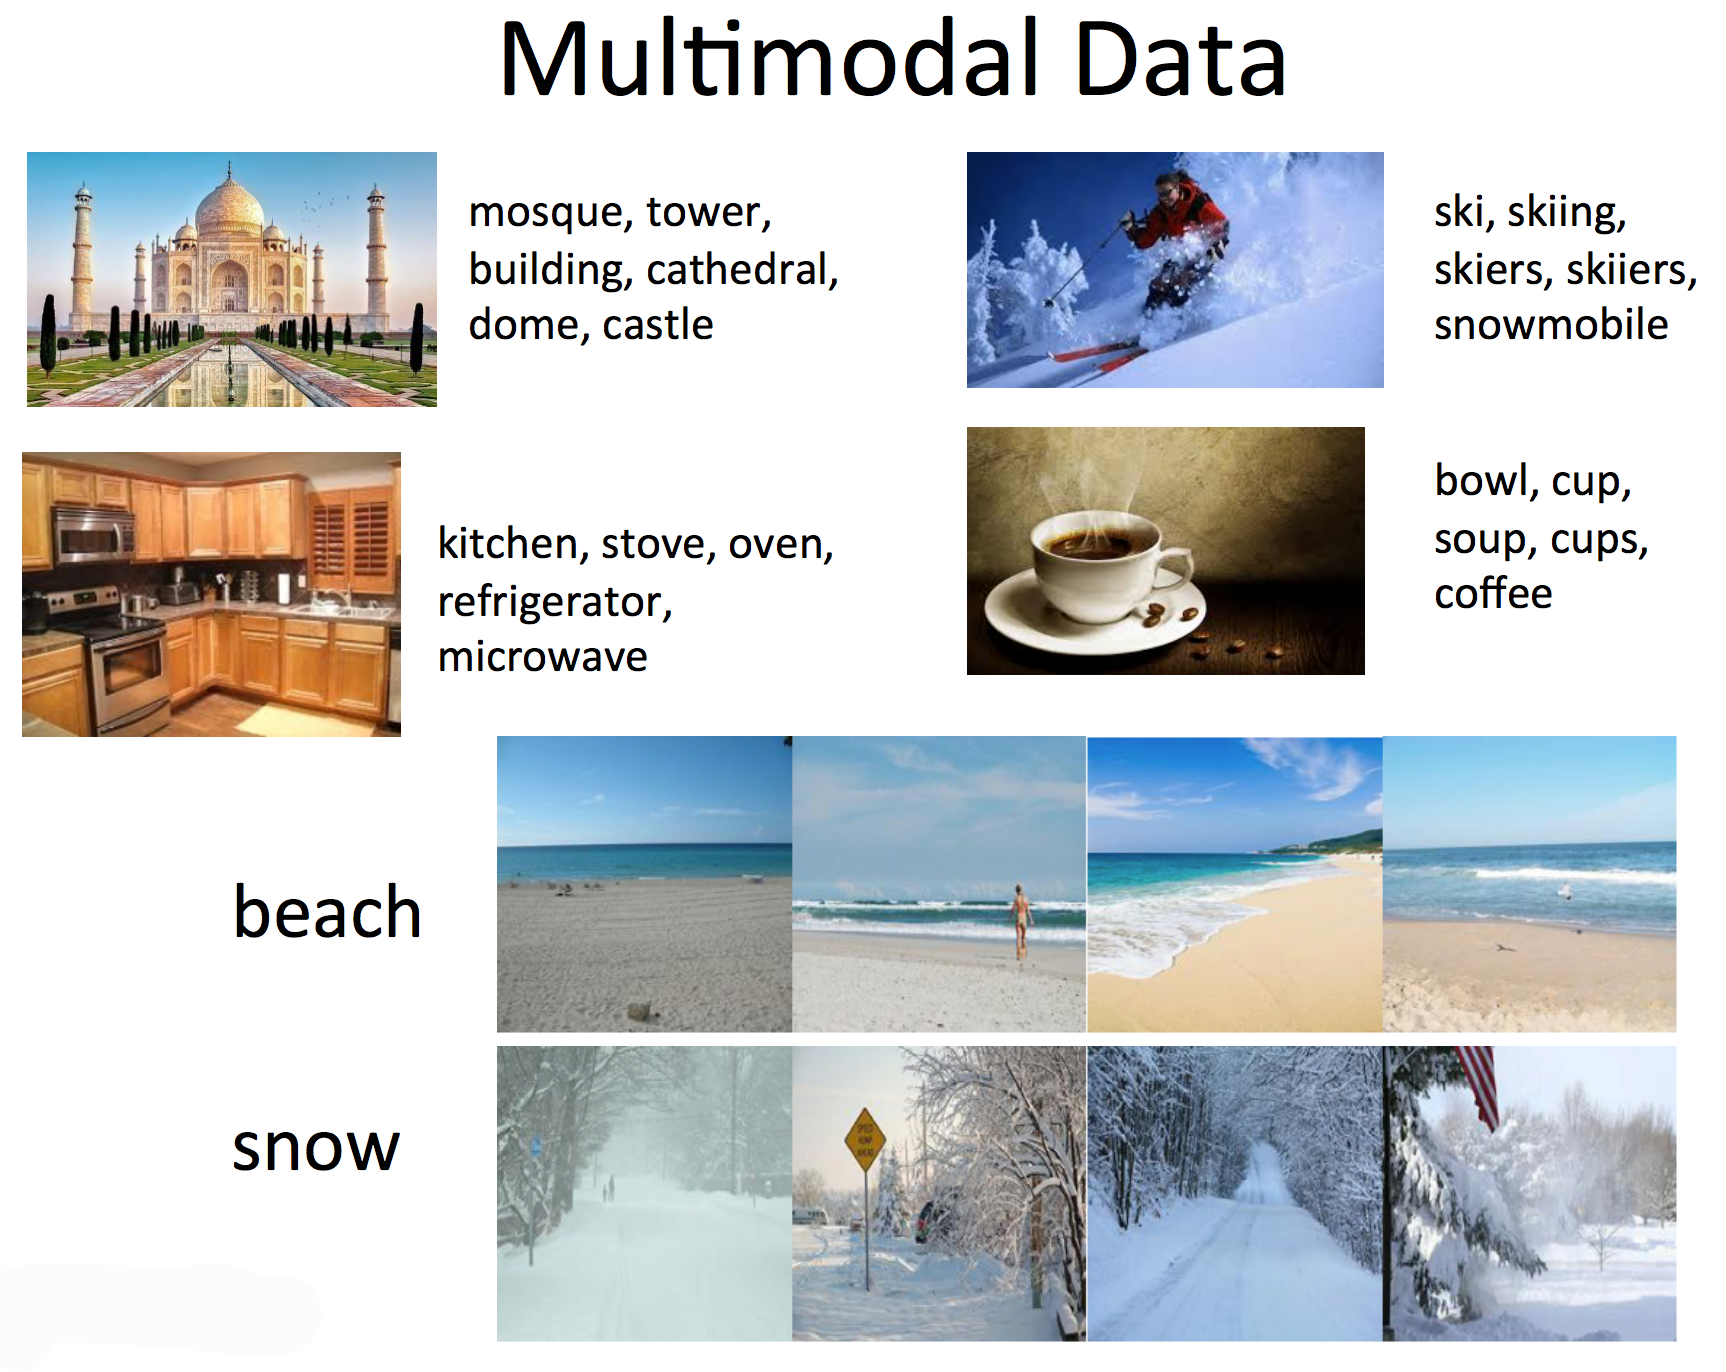
\includegraphics[width=0.7\textwidth]{images/multimodal1.png}
	\caption{Images from text \footnote{Ryan Kiros, 2014},\\ \url{http://videolectures.net/kdd2014_salakhutdinov_deep_learning/}}
\end{figure} 

\end{frame}


\begin{frame}{Multimodal data, \#2}

\begin{figure}[h!]
	\centering
	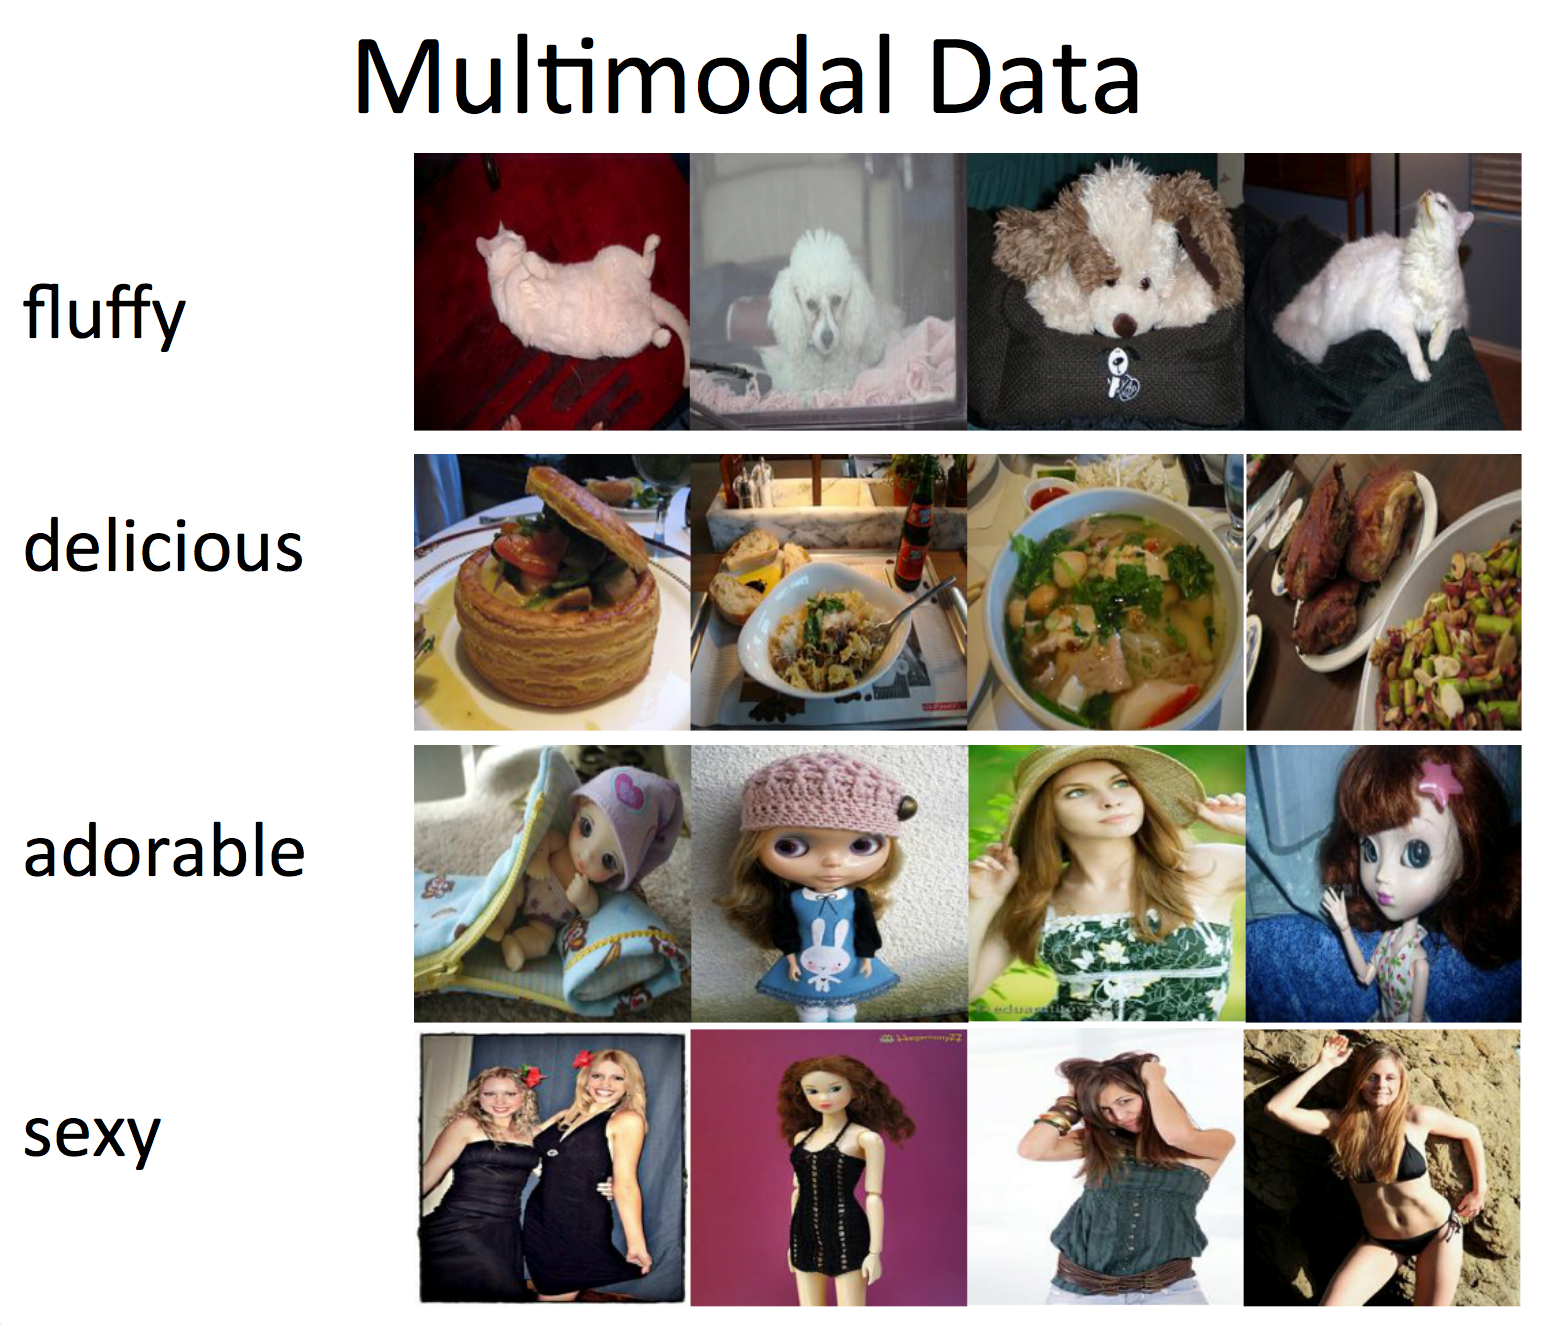
\includegraphics[width=0.7\textwidth]{images/multimodal2.png}
	\caption{Images from text \footnote{Ryan Kiros, 2014},\\ \url{http://videolectures.net/kdd2014_salakhutdinov_deep_learning/}}
\end{figure} 

\end{frame}


\begin{frame}{Text from images}

\begin{figure}[h!]
	\centering
	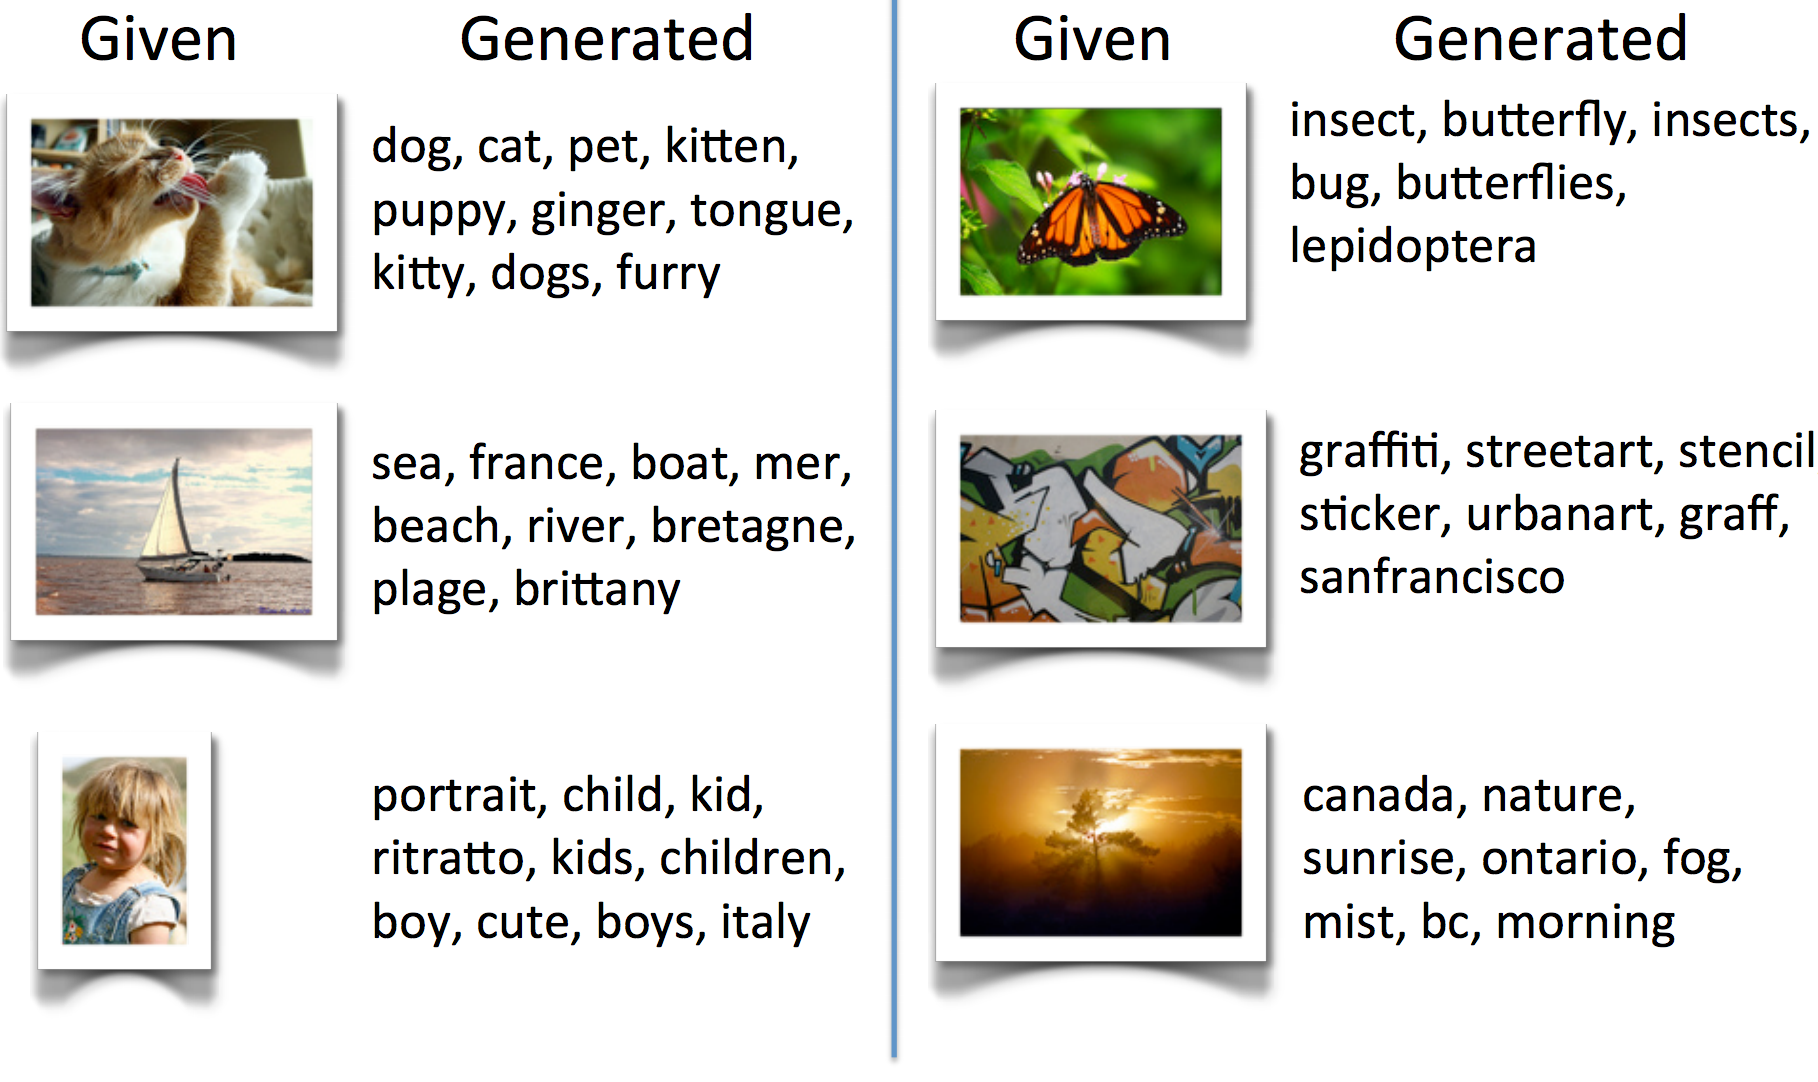
\includegraphics[width=1\textwidth]{images/text_generation.png}
	\caption{Text Generated from	 Images \\ \url{http://videolectures.net/kdd2014_salakhutdinov_deep_learning/}}
\end{figure} 

\end{frame}


\begin{frame}{Natural language from image}

\begin{figure}[h!]
	\centering
	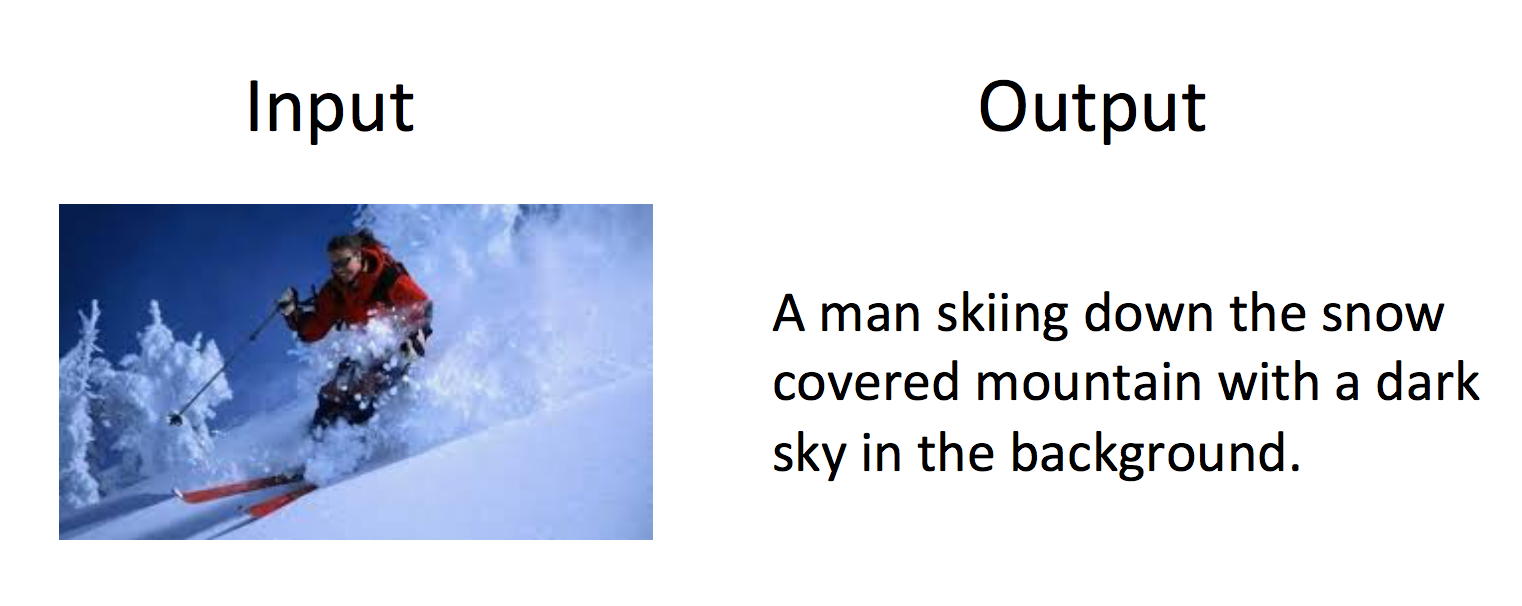
\includegraphics[width=0.7\textwidth]{images/nl_generation.png}
	\caption{Natural Text Generated from	 Images \\ \url{http://videolectures.net/kdd2014_salakhutdinov_deep_learning/}}
\end{figure} 

\end{frame}


\begin{frame}{Multimodal Linguistic Regularities, \#1}

\begin{figure}[h!]
	\centering
	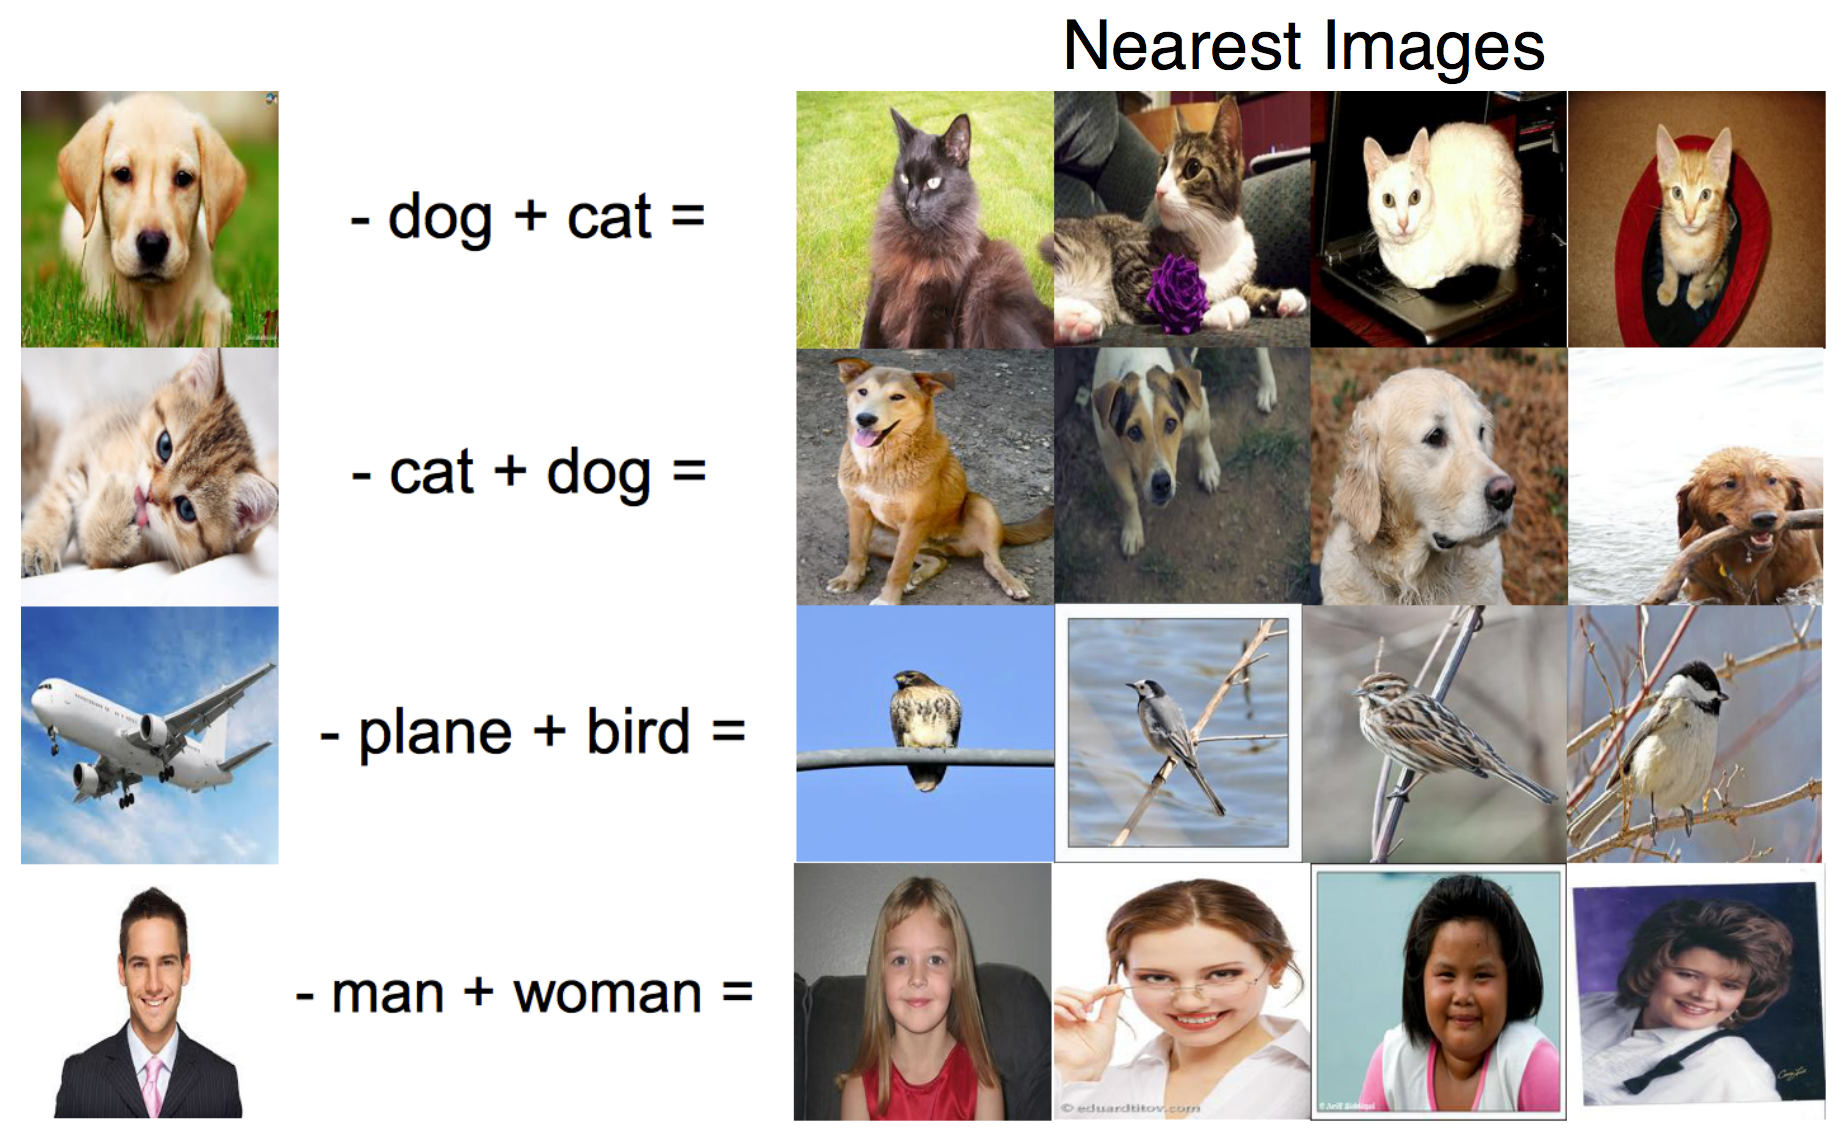
\includegraphics[width=1\textwidth]{images/mlr1.png}
	\caption{Multimodal Linguistic Regularities \footnote{Ryan Kiros, 2014},\\ \url{http://videolectures.net/kdd2014_salakhutdinov_deep_learning/}}
\end{figure} 

\end{frame}


\begin{frame}{Multimodal Linguistic Regularities, \#2}

\begin{figure}[h!]
	\centering
	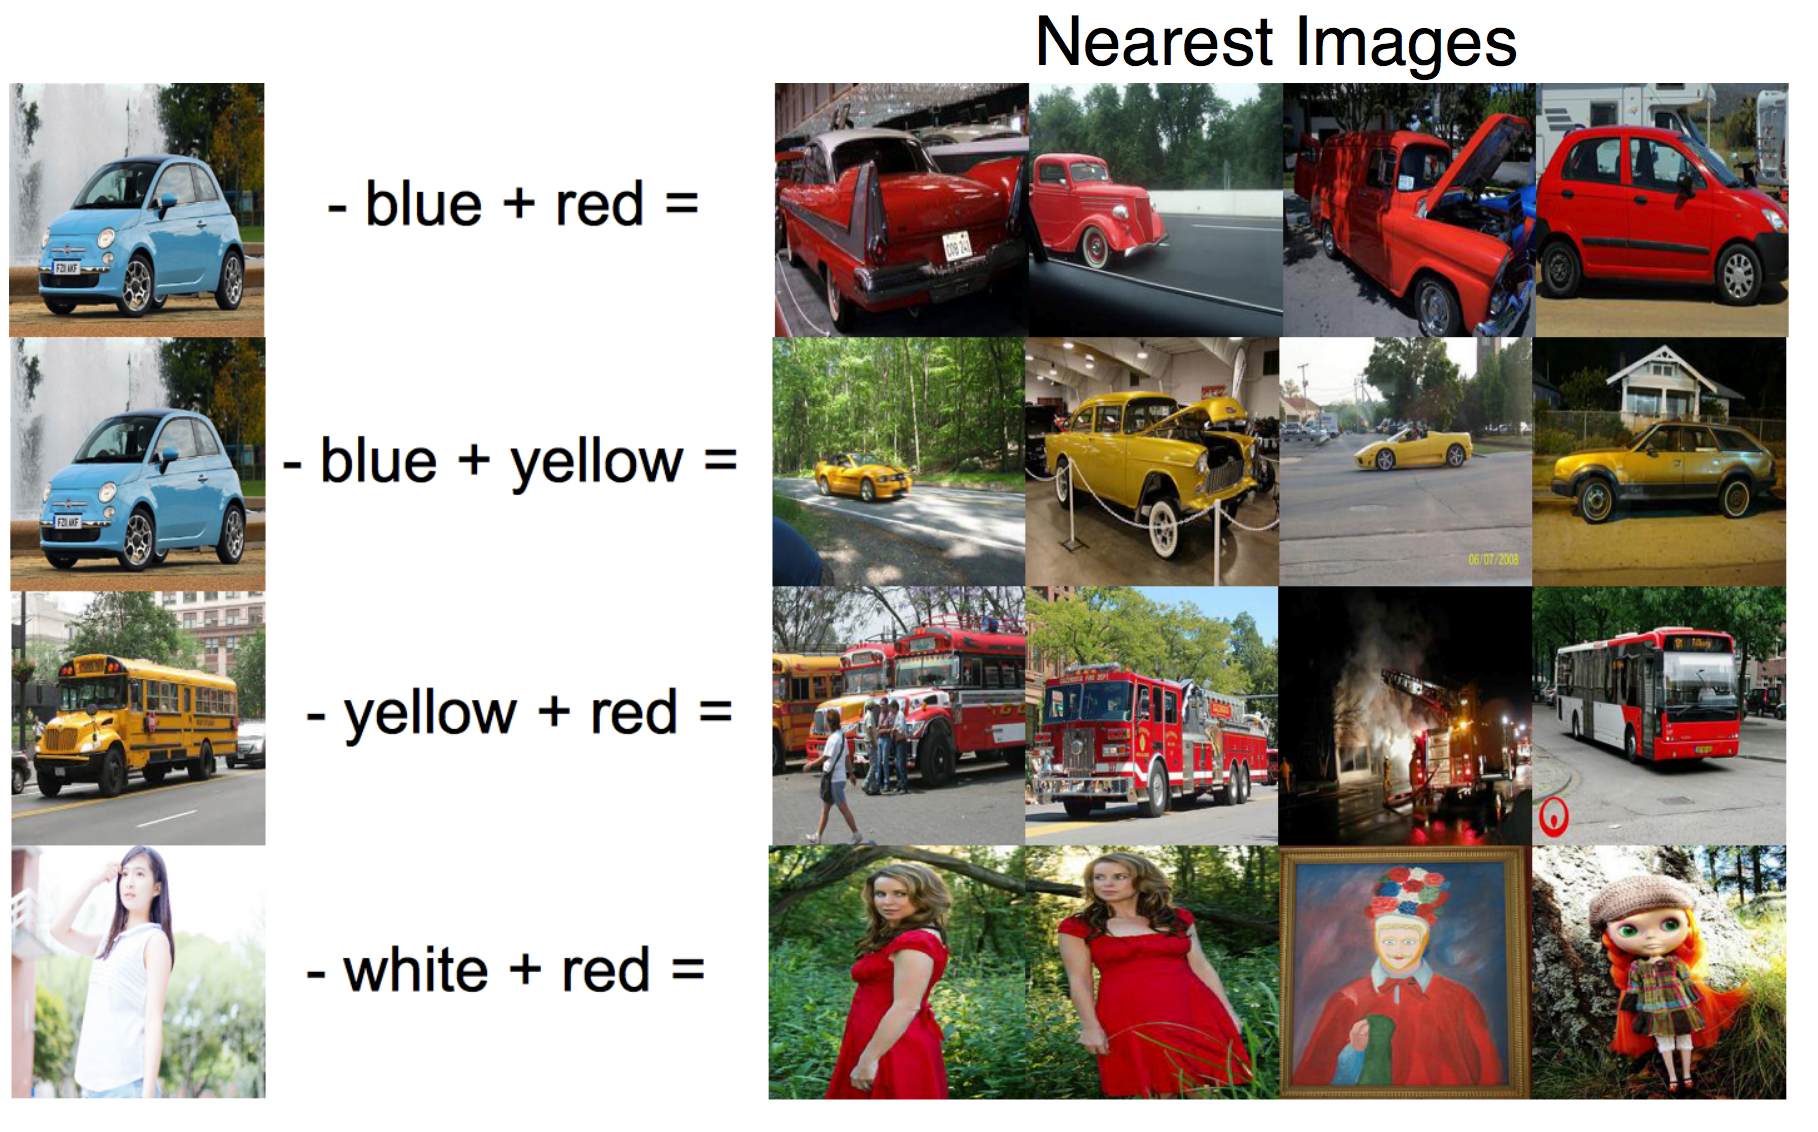
\includegraphics[width=1\textwidth]{images/mlr2.png}
	\caption{Multimodal Linguistic Regularities \footnote{Ryan Kiros, 2014},\\ \url{http://videolectures.net/kdd2014_salakhutdinov_deep_learning/}}
\end{figure} 

\end{frame}


\begin{frame}[plain]
\begin{center}
{\Large Вопросы}
\end{center}
\end{frame}

\end{document}
